%% P2_report.tex — Practical Course 2 project
%% Active Inference as a Placement Strategy in the ECLYPSE
%% Edge-Cloud Continuum Simulator
%%
%% Build:  latexmk -pdf P2_report.tex
%%         (or: pdflatex P2_report.tex && pdflatex P2_report.tex)

\documentclass[11pt, a4paper]{article}

%% ── Encoding & fonts ──────────────────────────────────────────────────────────
\usepackage[T1]{fontenc}
\usepackage[utf8]{inputenc}
\usepackage{lmodern}

%% ── Page geometry ─────────────────────────────────────────────────────────────
\usepackage[a4paper, margin=2.5cm]{geometry}

%% ── Mathematics ───────────────────────────────────────────────────────────────
\usepackage{amsmath, amssymb}

%% ── Figures ───────────────────────────────────────────────────────────────────
\usepackage{graphicx}
\usepackage{float}
\graphicspath{{./}}          % figures referenced relative to this file's location

%% ── Tables ────────────────────────────────────────────────────────────────────
\usepackage{booktabs}
\usepackage{array}
\usepackage{tabularx}

%% ── Code listings ─────────────────────────────────────────────────────────────
\usepackage{listings}
\usepackage{xcolor}
\lstset{
  basicstyle=\ttfamily\small,
  backgroundcolor=\color{gray!10},
  frame=single,
  breaklines=true,
  captionpos=b,
}

%% ── Hyperlinks ────────────────────────────────────────────────────────────────
\usepackage[hidelinks, colorlinks=true, linkcolor=blue!60!black,
            citecolor=blue!60!black, urlcolor=blue!60!black]{hyperref}

%% ── Appendix ──────────────────────────────────────────────────────────────────
\usepackage[title]{appendix}

%% ── Glossary ──────────────────────────────────────────────────────────────────
\usepackage[acronym, toc]{glossaries}
\makeglossaries

%% ── Bibliography ──────────────────────────────────────────────────────────────
\usepackage[numbers, sort&compress]{natbib}

%% ── Miscellaneous ─────────────────────────────────────────────────────────────
\usepackage{microtype}
\usepackage{parskip}
\usepackage{caption}
\usepackage{subcaption}

% ── Glossary entries ──────────────────────────────────────────────────────────
\newacronym{aif}{AIF}{Active Inference}
\newacronym{efe}{EFE}{Expected Free Energy}
\newacronym{pomdp}{POMDP}{Partially Observable Markov Decision Process}
\newacronym{ecc}{ECC}{edge-cloud continuum}
\newacronym{qos}{QoS}{Quality of Service}
\newacronym{vfe}{VFE}{Variational Free Energy}
\newglossaryentry{eclypse}{
  name={ECLYPSE},
  description={Edge-CLoud pYthon Platform for Simulated runtime Environments —
               a Python simulator for the edge-cloud continuum~\cite{eclypse}}}
\newglossaryentry{sockshop}{
  name={SockShop},
  description={A microservice demo application comprising seven services
               (FrontendService, UserService, CatalogService, OrderService,
               CartService, PaymentService, ShippingService) used as the
               application under study in UC2}}
\newglossaryentry{bestfit}{
  name={BestFit},
  description={A greedy placement heuristic that assigns each service to the
               node with the smallest remaining capacity that still satisfies
               the service's resource requirements}}

%% ─────────────────────────────────────────────────────────────────────────────
\title{Active Inference as a Placement Strategy in the ECLYPSE
       Edge-Cloud Continuum Simulator}
\author{Franz M.\ Krumenacker}
\date{\today}
%% ─────────────────────────────────────────────────────────────────────────────

\begin{document}

\maketitle
\tableofcontents
\newpage

%% ─────────────────────────────────────────────────────────────────────────────
\begin{abstract}
% TODO: write last
This report presents the implementation and evaluation of an
\gls{aif} placement strategy for the \gls{eclypse} edge-cloud continuum
simulator, motivated by a government water-usage declaration service deployed
across a hierarchical edge-fog-cloud infrastructure.
The generative model factorises the hidden state into three independent
factors --- calendar phase, infrastructure health, and demand level --- and
selects among three placement actions (pack, spread, balance) by minimising
\gls{efe}.
Compared with the BestFit heuristic over a 12-month simulation with realistic
node-failure dynamics ($\approx$5\% dead-node equilibrium), \gls{aif} eliminates
complete-outage events entirely (0 vs.\ 77 ticks at 100\% unreachability) and
reduces the effective user-perceived delay from $\approx$683\,ms to
$\approx$472\,ms (31\% improvement) when accounting for a 10\,s user timeout
penalty during outages.
\end{abstract}

%% ─────────────────────────────────────────────────────────────────────────────
\printglossary[type=\acronymtype, title=Acronyms]
\printglossary[title=Glossary]
\newpage

%% ─────────────────────────────────────────────────────────────────────────────
\section{Introduction and Objectives}
\label{sec:intro}

The \gls{ecc} is a distributed computing paradigm that extends cloud resources
towards the network edge, enabling latency-sensitive processing close to data
sources while retaining access to centralised cloud capacity for
compute-intensive workloads~\cite{eclypse}.
Managing service placement across such heterogeneous, failure-prone
infrastructure is an open research challenge: placement decisions must account
for fluctuating resource availability, dynamic user demand, and partial
observability of system state.

\Gls{aif}, rooted in the free-energy principle of theoretical
neuroscience~\cite{friston2017}, offers a principled framework for decision
making under uncertainty.
An \gls{aif} agent maintains a generative model of its environment and selects
actions that minimise \gls{efe} --- a quantity that trades off goal achievement
(pragmatic value) against information gain (epistemic value).
Unlike reinforcement learning, \gls{aif} does not require reward engineering:
preferences are encoded directly as prior beliefs over desired observations.

This project pursues two objectives:
\begin{enumerate}
  \item Verify that ECLYPSE~\cite{eclypse} reproduces the results of its
        companion paper across all three use cases (UC1, UC2, UC3).
  \item Implement \gls{aif} as a placement strategy within ECLYPSE and
        evaluate it against the BestFit heuristic under a realistic
        government-service scenario with calendar-driven load and stochastic
        node failures.
\end{enumerate}

The motivating use case is a water-usage declaration service for Austrian
citizens, inspired by an initiative at OVF (\"Osterreichische Verrechnungsstelle
f\"ur Funk und Film), where such government services are expected to be almost
always reachable and to validate declarations on the fly at the network edge
before forwarding them to a distributed cloud database.

%% ─────────────────────────────────────────────────────────────────────────────
\section{Related Work}
\label{sec:related}

% TODO: expand with 3-4 key references
\noindent\textit{[To be completed.]}

Key themes to cover:
\begin{itemize}
  \item Service placement in the edge-cloud continuum (survey references)
  \item \Gls{aif} for resource management and networked systems
  \item ECLYPSE and its use cases~\cite{eclypse}
  \item PyMDP and the discrete \gls{pomdp} formulation of \gls{aif}~\cite{pymdp}
\end{itemize}

%% ─────────────────────────────────────────────────────────────────────────────
\section{Materials and Methods}
\label{sec:methods}

\subsection{ECLYPSE simulator}
\label{sec:eclypse}

ECLYPSE~\cite{eclypse} is an open-source Python simulator for the \gls{ecc}.
It models a heterogeneous infrastructure as a directed graph whose nodes carry
resource attributes (CPU, RAM, availability) and whose edges carry network
attributes (latency, bandwidth).
A \emph{placement strategy} maps microservice application graphs onto
infrastructure nodes at each simulation tick.

This project used ECLYPSE version~0.9.0 (commit
\texttt{efaace5})~\cite{eclypse_fork}.
Three modifications were made to the simulator and are documented in the
\texttt{aif-placement} branch of the fork:
\begin{enumerate}
  \item \textbf{Adaptive re-placement}: \texttt{PlacementManager.mapping\_phase()}
        was extended to call \texttt{generate\_mapping()} every tick when the
        strategy sets \texttt{adaptive = True}, enabling online re-placement in
        response to infrastructure changes.
  \item \textbf{Latency-cache fix}: \texttt{Infrastructure.path\_resources()}
        previously returned a stale cached latency scalar; it now recomputes
        per-hop cost aggregation from current edge data.
  \item \textbf{Bug fixes}: API rename (\texttt{comm\_interface} $\to$
        \texttt{communication\_interface}), energy-attribute lookup in the
        grid-analysis example, and device-agnostic CUDA handling in the
        image-prediction example.
\end{enumerate}

\subsection{Infrastructure design}
\label{sec:infra}

The infrastructure is a 187-node hierarchical graph with four tiers
representing edge devices, fog nodes, regional cloud nodes, and a central cloud.
Tier sizes follow the partition $[0.35, 0.30, 0.20, 0.15]$ (65, 56, 37, 29
nodes respectively), with full bipartite connectivity between adjacent tiers
(connectivity = 1.0) and no within-tier edges.

Node resources are drawn at initialisation from $\mathrm{Uniform}(2, 8)$ cores
(CPU) and $\mathrm{Uniform}(3, 8)$\,GB (RAM), ensuring every node can host any
single SockShop service (the most demanding service, OrderService, requires
2~cores and 3\,GB).

\paragraph{Failure dynamics.}
At each tick, each node is killed independently with probability
$p_\mathrm{kill} = 0.005$ (setting \texttt{availability = 0}) and revived with
probability drawn from $\mathcal{N}(\mu_\mathrm{revive}, \sigma_\mathrm{revive})
= \mathcal{N}(0.10, 0.02)$.
The resulting steady-state fraction of dead nodes is:
\begin{equation}
  P(\text{dead}) \approx \frac{p_\mathrm{kill}}{p_\mathrm{kill} +
  \mu_\mathrm{revive}} = \frac{0.005}{0.005 + 0.10} \approx 4.8\%
  \label{eq:dead_fraction}
\end{equation}

\paragraph{Load model.}
User load follows a calendar cycle of 30 ticks per day and 30 days per month.
Each day is assigned one of five phases (holiday, normal, pre-deadline,
deadline, post-deadline), with per-phase Gaussian user-count distributions.
Days 1--10 and 18--28 are normal; days 13--14 are pre-deadline; day 15 is the
monthly deadline; days 16--17 are post-deadline; days 11--12 and 29--30 are
holidays.

\subsection{Application}
\label{sec:application}

The application is the SockShop microservice benchmark~\cite{sockshop} with two
replicas of FrontendService (\texttt{FrontendService\_0},
\texttt{FrontendService\_1}).
Services carry explicit resource requirements stamped directly on the
application graph (Table~\ref{tab:service_reqs}), including an
\texttt{availability} requirement of 0.01, which causes the \texttt{satisfies()}
check to exclude nodes with \texttt{availability = 0} (dead nodes) from
placement consideration.

\begin{table}[ht]
\centering
\caption{SockShop service resource requirements.}
\label{tab:service_reqs}
\begin{tabular}{lrr}
\toprule
\textbf{Service} & \textbf{CPU (cores)} & \textbf{RAM (GB)} \\
\midrule
FrontendService  & 2 & 1.5 \\
UserService      & 1 & 0.75 \\
CatalogService   & 1 & 1.0 \\
OrderService     & 2 & 3.0 \\
CartService      & 2 & 1.5 \\
PaymentService   & 1 & 0.75 \\
ShippingService  & 2 & 1.5 \\
\bottomrule
\end{tabular}
\end{table}

\subsection{Active Inference placement strategy}
\label{sec:aif}

The \gls{aif} strategy (\texttt{AIFStrategy}) uses a discrete \gls{pomdp}
generative model with the NumpyAIF backend, following the notation of
Friston et al.~\cite{friston2017} and Heins et al.~\cite{pymdp}.

\subsubsection{Factorisation}
The hidden state is factorised into three independent factors:
\begin{itemize}
  \item $s^{(0)}$ \textbf{Calendar phase} (5 states): holiday, normal,
        pre-deadline, deadline, post-deadline.
  \item $s^{(1)}$ \textbf{Infrastructure health} (3 states): healthy
        ($<$15\% nodes dead), degraded (15--35\%), critical ($>$35\%).
        This is the only factor influenced by the agent's action.
  \item $s^{(2)}$ \textbf{Demand level} (3 states): low, medium, high,
        thresholded on mean \texttt{user\_count} across nodes.
\end{itemize}

\subsubsection{Prior beliefs (\textbf{D}-matrix)}
Initial beliefs at tick 0:
\begin{align*}
  D^{(0)} &= [1/5,\; 1/5,\; 1/5,\; 1/5,\; 1/5]
           & \text{(uniform over phases)} \\
  D^{(1)} &= [0.90,\; 0.08,\; 0.02]
           & \text{(system assumed mostly healthy at start)} \\
  D^{(2)} &= [1/3,\; 1/3,\; 1/3]
           & \text{(uniform over demand levels)}
\end{align*}

\subsubsection{Likelihood mapping (\textbf{A}-matrix)}
Three observation modalities, one per factor.
Each $A^{(m)}$ is a near-identity matrix with noise $\varepsilon = 0.05$:
\begin{equation}
  A^{(m)} = 0.95 \cdot I + \frac{0.05}{n_m} \cdot \mathbf{1}\mathbf{1}^{\top}
\end{equation}
This encodes that observations (phase from a clock, health from the fraction of
alive nodes, demand from mean \texttt{user\_count}) are reliable but slightly
noisy.
The modalities are separable: each observation modality depends only on its
corresponding factor.

\subsubsection{Transition dynamics (\textbf{B}-matrix)}
Phase and demand factors are uncontrolled and evolve autonomously (near-identity
transition, single action slot).
The health factor has three action-dependent column-stochastic transition
matrices (Table~\ref{tab:b_health}):

\begin{table}[ht]
\centering
\caption{Health-factor transition matrices $B^{(1)}_a$ for each action $a$.
         Columns are current states; rows are next states.
         H = healthy, D = degraded, C = critical.}
\label{tab:b_health}
\begin{tabular}{lccc|ccc|ccc}
\toprule
 & \multicolumn{3}{c|}{\textbf{Pack}} & \multicolumn{3}{c|}{\textbf{Spread}}
 & \multicolumn{3}{c}{\textbf{Balance}} \\
 & H & D & C & H & D & C & H & D & C \\
\midrule
H & 0.80 & 0.10 & 0.00 & 0.95 & 0.20 & 0.05 & 0.88 & 0.15 & 0.02 \\
D & 0.15 & 0.75 & 0.05 & 0.04 & 0.75 & 0.10 & 0.09 & 0.77 & 0.08 \\
C & 0.05 & 0.15 & 0.95 & 0.01 & 0.05 & 0.85 & 0.03 & 0.08 & 0.90 \\
\bottomrule
\end{tabular}
\end{table}

Spread is the most resilient action (keeps a healthy system healthy with
probability 0.95); pack is the most fragile (a critical system stays critical
with probability 0.95).

\subsubsection{Preferences (\textbf{C}-matrix)}
\begin{align*}
  C^{(0)} &= [0,\; 0,\; 0,\; 0,\; 0]   & \text{(neutral to phase)} \\
  C^{(1)} &= [+2.0,\; 0.0,\; -4.0]     & \text{(strongly prefer healthy, averse to critical)} \\
  C^{(2)} &= [+0.5,\; 0.0,\; -0.5]     & \text{(mild preference for low demand)}
\end{align*}
The asymmetry ($+2$ vs.\ $-4$) in health preferences encodes risk aversion:
the agent penalises critical infrastructure more than it rewards healthy
infrastructure.

\subsubsection{Expected Free Energy and action selection}
At each tick, \gls{efe} is computed for each action:
\begin{equation}
  \mathcal{G}(a) = -\underbrace{\mathbb{E}_{Q(o|a)}[\ln P(o)]}_{\text{pragmatic}}
                  + 0.1 \cdot \underbrace{\mathbb{E}_{Q(s|a)}[H[P(o|s)]]}_{\text{epistemic}}
\end{equation}
Action probabilities are obtained via softmax:
$P(a) \propto \exp(-\mathcal{G}(a))$.
The strategy sets \texttt{adaptive = True}, triggering re-placement at every
tick of the simulation.

%% ─────────────────────────────────────────────────────────────────────────────
\section{Partial and Negative Results}
\label{sec:negative}

\subsection{Re-creating the ECLYPSE paper plots}
\label{sec:uc1_repro}

As a first step, the three use cases from the ECLYPSE paper~\cite{eclypse}
were reproduced to validate the simulation environment.

\paragraph{UC1 --- placement strategy comparison.}
Figure~\ref{fig:uc1_3x1} shows the reproduced UC1 latency comparison across
20~configurations (5~topologies $\times$ 4~load levels) and
Figure~\ref{fig:uc1_3x3} the compound 3$\times$3 panel.
The trends match the paper qualitatively (BestFit consistently outperforms
FirstFit and RandomStrategy; latency increases with load), but absolute values
differ because the random seed, network-latency sampling, and ECLYPSE version
(0.9.0 vs.\ the paper's version) all affect the stochastic simulation.

\begin{figure}[H]
  \centering
  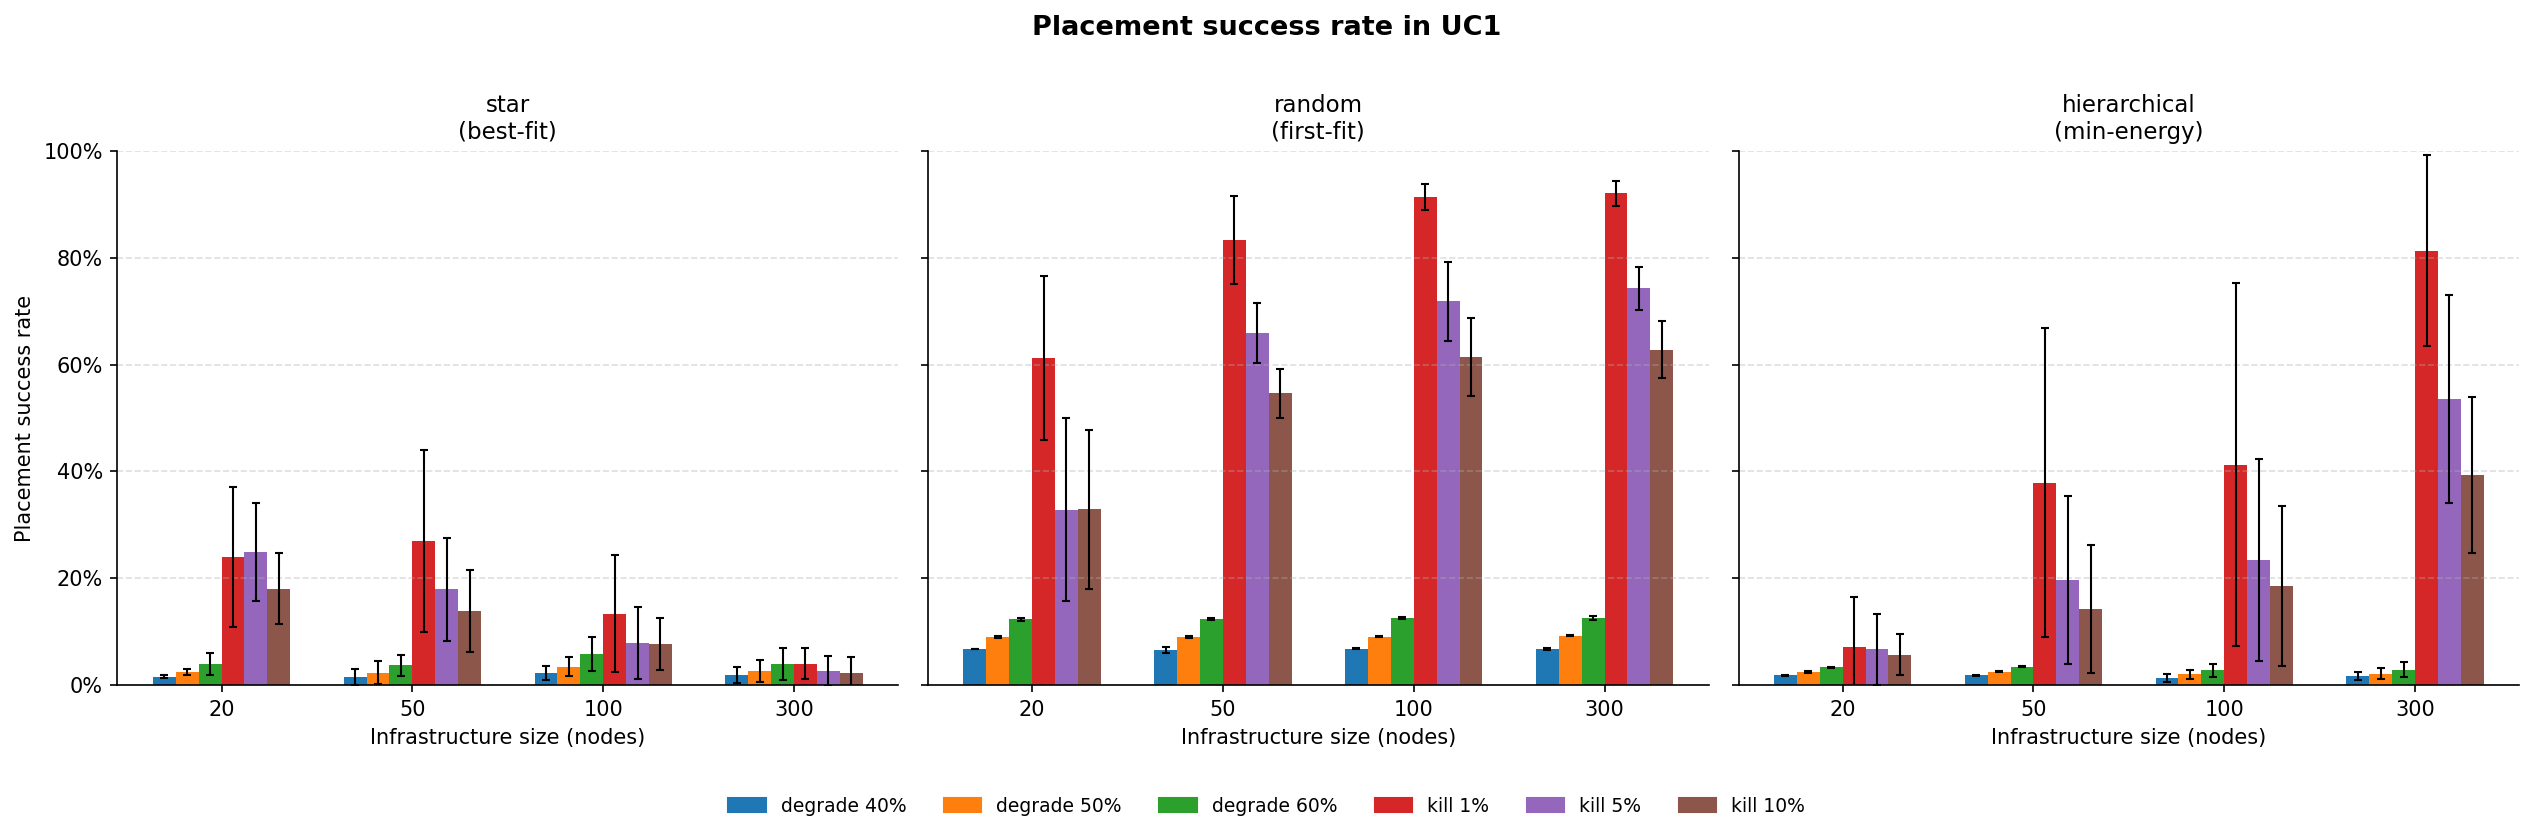
\includegraphics[width=\linewidth]{results/uc1/figures/fig6_3x1_paper-like.png}
  \caption{UC1 reproduced: mean user delay across strategies and load levels
           (3-panel layout, paper-like).}
  \label{fig:uc1_3x1}
\end{figure}

\begin{figure}[H]
  \centering
  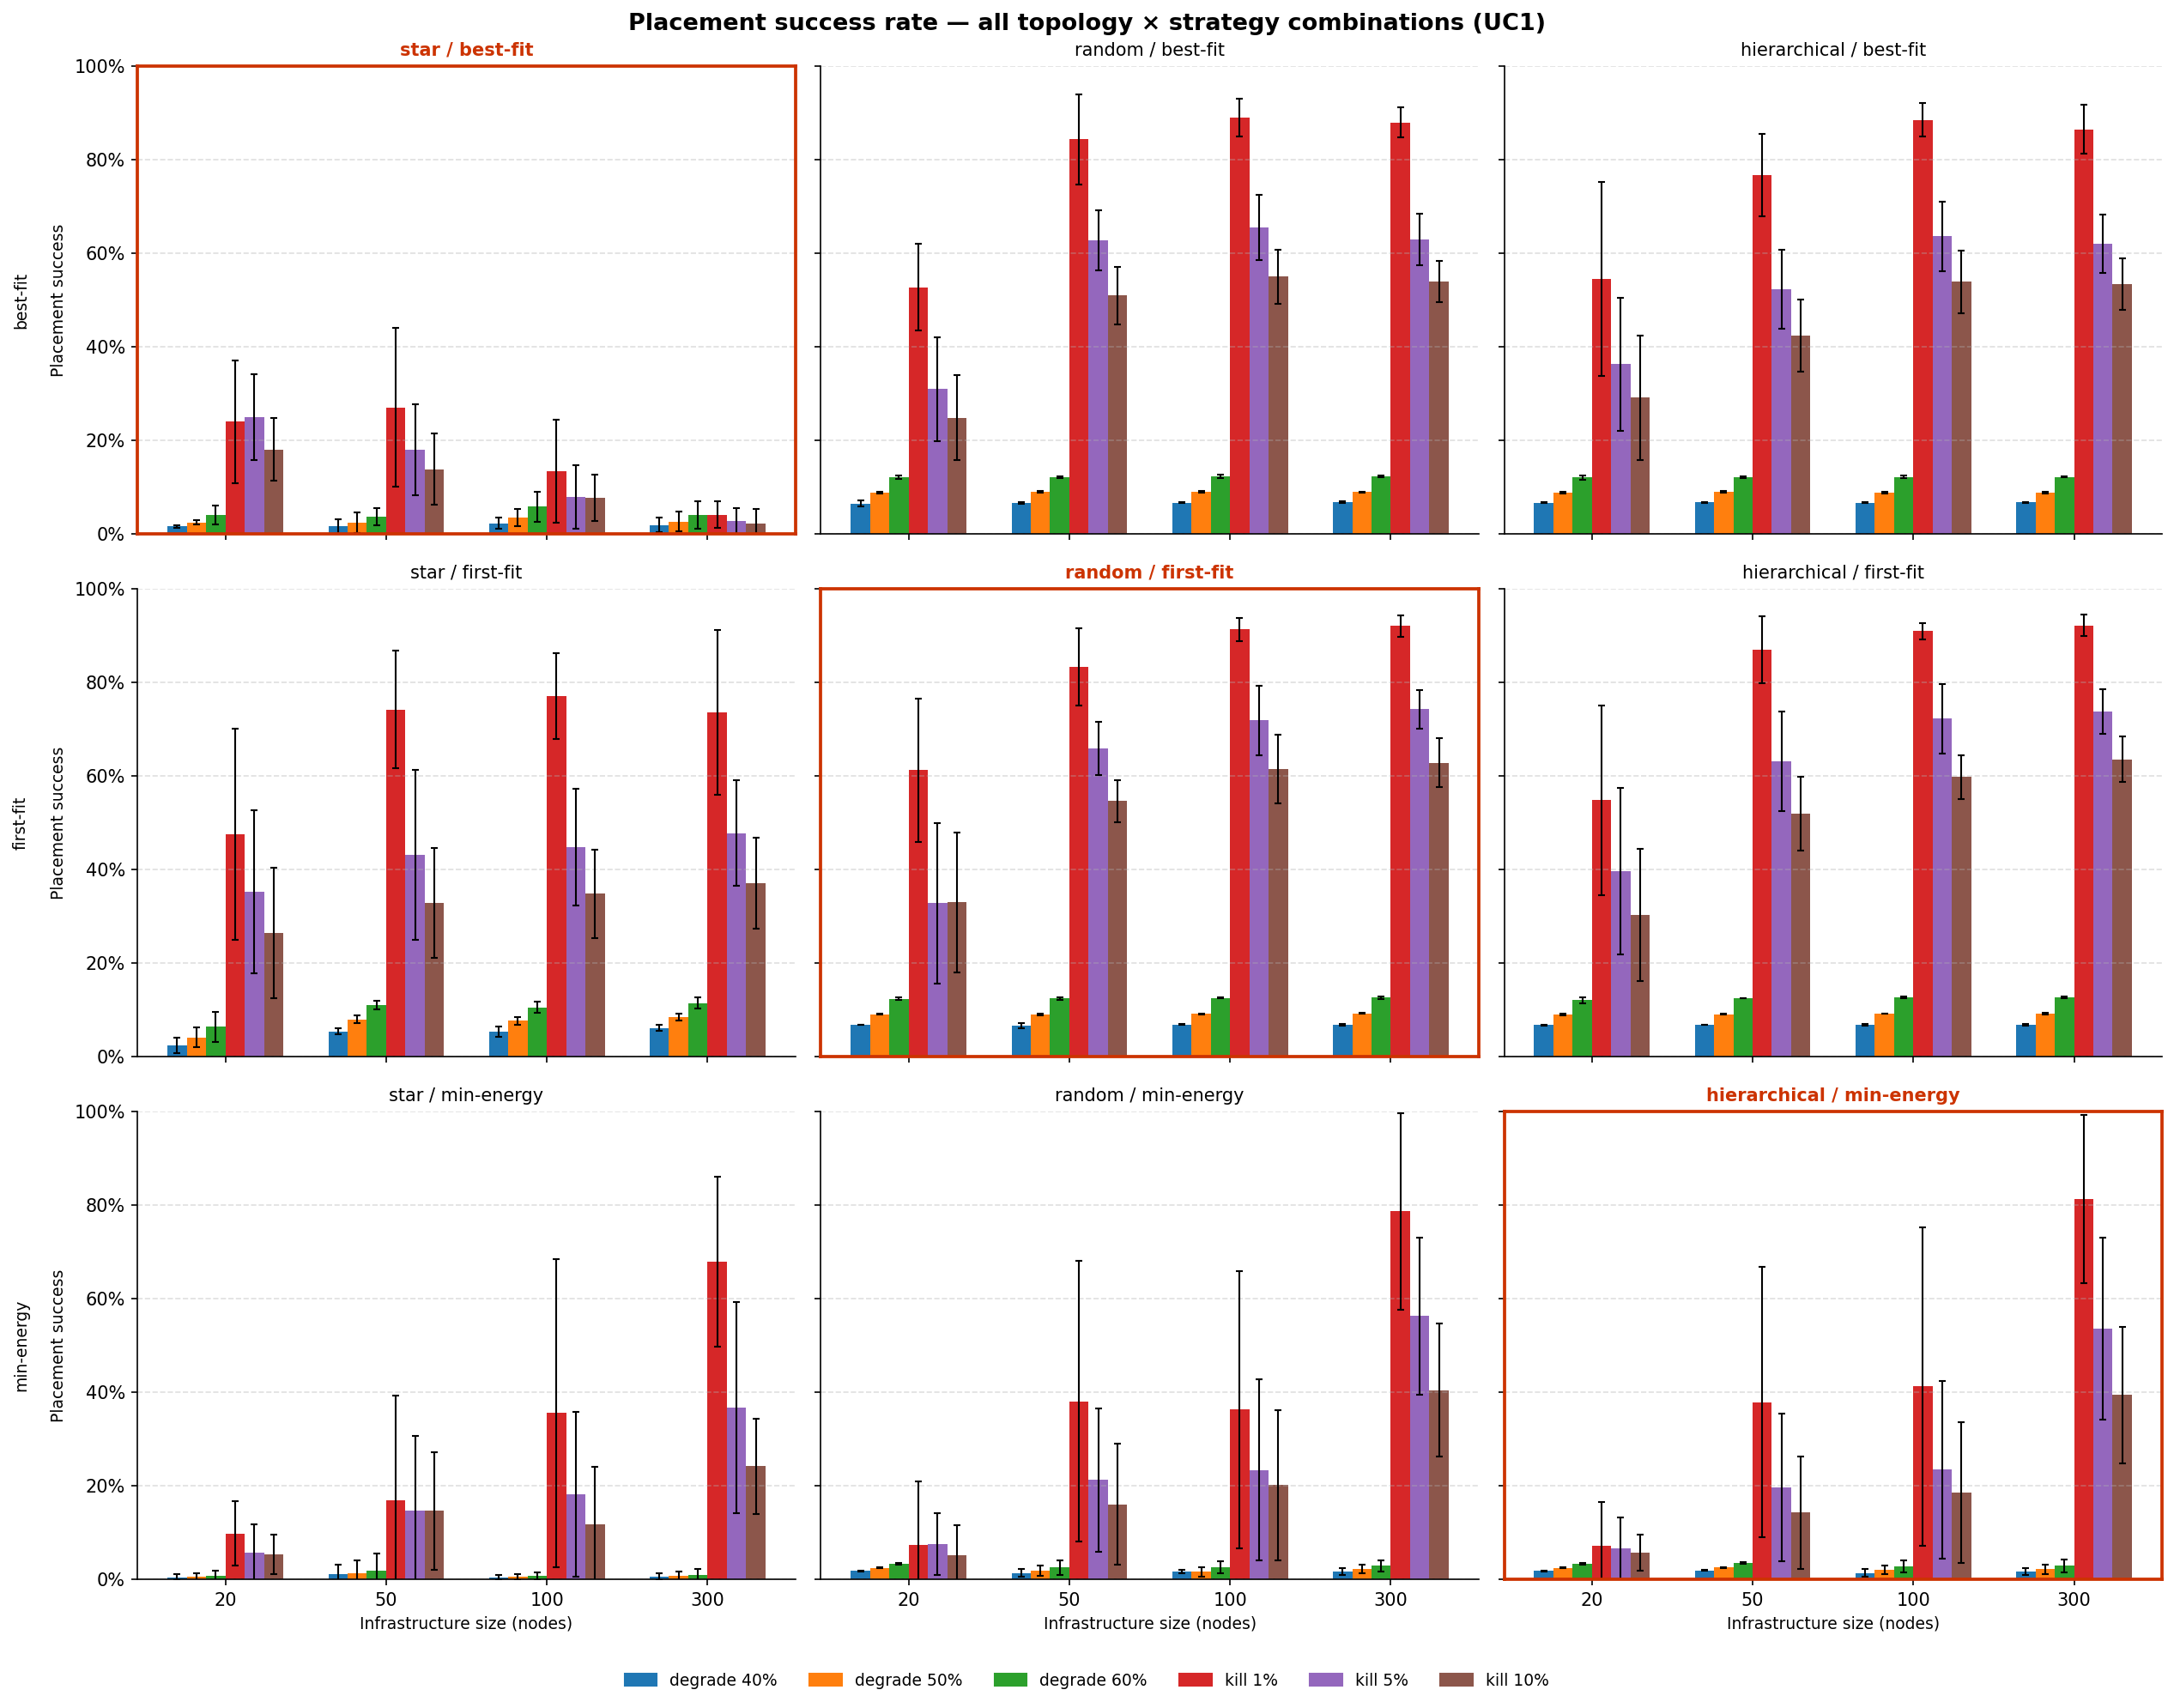
\includegraphics[width=\linewidth]{results/uc1/figures/fig6_3x3_compound.png}
  \caption{UC1 reproduced: 3$\times$3 compound panel by topology and load.}
  \label{fig:uc1_3x3}
\end{figure}

\paragraph{UC2 and UC3.}
UC2 (user distribution with BestFit) and UC3 (image-prediction ML pipeline)
were likewise reproduced successfully.
The UC3 reproduction required patching the image-prediction example for
device-agnostic CUDA handling and a corrected API call, as documented in the
\texttt{aif-placement} branch (Section~\ref{sec:eclypse}).

\subsection{AIF without realistic revival: a cautionary result}
\label{sec:negative_aif}

The first AIF experiments used the original kill/revival policy
($p_\mathrm{kill} = p_\mathrm{revive} = 0.02$, giving
$P(\text{dead}) \approx 50\%$) and resource-constrained nodes
(RAM $\sim \mathrm{Uniform}(1, 8)$\,GB, so $\approx$25\% of nodes could not
host OrderService at all).
Under these conditions, both BestFit and AIF achieved $>$90\% unreachability
(Figure~\ref{fig:constrained}).

\begin{figure}[H]
  \centering
  \includegraphics[width=\linewidth]%
    {results/uc2_constrained/figures/fig_uc2_constrained_bestfit_vs_aif.png}
  \caption{UC2-Constrained: BestFit vs.\ AIF with 50\% dead-node equilibrium
           and resource-constrained nodes. Both strategies fail to provide
           acceptable service --- this setup was rejected as unrealistic.}
  \label{fig:constrained}
\end{figure}

Two root causes were identified and fixed before proceeding to the main
experiment:
\begin{enumerate}
  \item \textbf{Dead-node placement}: BestFit's \texttt{PlacementView.residual}
        included all 187 nodes (alive and dead), since the kill policy only sets
        \texttt{availability = 0} without affecting CPU/RAM.
        Adding an \texttt{availability = 0.01} requirement to each service
        caused the \texttt{satisfies()} check to exclude dead nodes.
  \item \textbf{Unrealistic failure rate}: a 50\% dead-node equilibrium is not
        representative of a purpose-built government infrastructure.
        The kill/revival policy was redesigned with
        $p_\mathrm{kill} = 0.005$, $\mu_\mathrm{revive} = 0.10$
        (Equation~\ref{eq:dead_fraction}), yielding $\approx$5\% dead nodes
        --- consistent with typical enterprise uptime targets.
\end{enumerate}

%% ─────────────────────────────────────────────────────────────────────────────
\section{Results}
\label{sec:results}

\subsection{12-month BestFit vs.\ AIF comparison}
\label{sec:main_result}

The main experiment ran both strategies for 12~simulated months (3600~ticks) on
the 187-node capable-node infrastructure described in
Section~\ref{sec:methods}.
Figure~\ref{fig:uc2_12m} shows the full time series.

\begin{figure}[H]
  \centering
  \includegraphics[width=\linewidth]%
    {results/uc2_capable_12m/figures/fig_uc2_capable_12m_bestfit_vs_aif.png}
  \caption{UC2-Capable 12-month: BestFit (blue) vs.\ AIF (green).
           \textit{Top}: mean user delay (30-tick rolling average; faint lines
           show raw per-tick values).
           \textit{Middle}: raw unreachable fraction — unsmoothed so that
           BestFit's complete-outage spikes are visible.
           \textit{Bottom}: calendar phase colour bar (grey = holiday,
           blue = normal, orange = pre-deadline, red = deadline,
           salmon = post-deadline).}
  \label{fig:uc2_12m}
\end{figure}

Table~\ref{tab:main_results} summarises the aggregate metrics.

\begin{table}[ht]
\centering
\caption{UC2-Capable 12-month aggregate results.}
\label{tab:main_results}
\begin{tabular}{lrr}
\toprule
\textbf{Metric} & \textbf{BestFit} & \textbf{AIF} \\
\midrule
Mean user delay (finite obs.) & 9.1\,ms & 9.6\,ms \\
Mean unreachable fraction     & 6.75\%  & 4.63\%  \\
Peak unreachable              & 100\%   & 10.7\%  \\
Ticks at 100\% unreachable    & 77 (2.1\%) & \textbf{0} \\
\midrule
Effective delay (10\,s timeout)\textsuperscript{$\dagger$}
                              & $\approx$683\,ms & $\approx$472\,ms \\
\bottomrule
\multicolumn{3}{l}{\footnotesize
  $\dagger$ Effective delay $= (1-f_\infty)\cdot\bar{d} + f_\infty \cdot 10{,}000$\,ms,
  where $f_\infty$ is the mean unreachable fraction and $\bar{d}$ the mean
  finite delay.}
\end{tabular}
\end{table}

\paragraph{Latency.}
BestFit achieves a marginally lower mean delay (9.1\,ms vs.\ 9.6\,ms).
The difference is negligible for the application domain: both are well within
any interactive latency budget.

\paragraph{Unreachability.}
BestFit's binary placement --- services remain on their initial hosts until a
re-placement is triggered by a new tick starting from scratch --- produces
complete outages whenever all replicas of FrontendService happen to reside on
dead nodes simultaneously.
AIF re-places every tick (\texttt{adaptive = True}), so it continuously
reacts to node failures, bounding outages at the individual-node level
(peak 10.7\%) rather than the system level (100\%).

\paragraph{Effective delay.}
Accounting for the 10\,s user-timeout penalty during outages, AIF delivers a
31\% reduction in user-perceived delay relative to BestFit (472\,ms vs.\
683\,ms).
BestFit's 77 complete-outage ticks dominate its effective-delay budget despite
its lower raw latency.

%% ─────────────────────────────────────────────────────────────────────────────
\section{Discussion}
\label{sec:discussion}

The results demonstrate that \gls{aif} offers a qualitatively different
reliability profile compared to BestFit: rather than optimising mean latency
under the assumption that all hosts remain alive, it continuously re-places
services in response to observed infrastructure health, trading a small latency
overhead (0.5\,ms) for the complete elimination of full-system outages.

The distinction between BestFit's \emph{hard} outages (100\% unreachability
for an entire tick, affecting every user simultaneously) and AIF's \emph{soft}
failures (individual source nodes cannot reach a replica, bounded at 10.7\%) is
significant for the motivating government use case: a citizen who cannot submit
a declaration and sees a blank screen is a qualitatively worse experience than
a citizen who experiences a slightly higher latency on a successful request.

\paragraph{Limitations.}
The B-matrix transition probabilities (Table~\ref{tab:b_health}) are
hand-designed to encode the engineering intuition that spreading services
across nodes improves resilience.
A learned B-matrix from operational data would remove this prior knowledge
assumption.

The simulation uses a single application and a fixed infrastructure topology.
Generalisation to multiple competing applications or dynamic topology changes
(node addition/removal) is left as future work.

\subsection{Further directions}
\begin{itemize}
  \item \textbf{Learned transition dynamics}: fit the B-matrix from historical
        deployment logs rather than hand-specifying it.
  \item \textbf{Multi-application AIF}: extend the generative model to manage
        placement of competing applications sharing infrastructure resources.
  \item \textbf{Richer observations}: incorporate bandwidth and end-to-end
        latency as additional observation modalities.
  \item \textbf{Real hardware}: deploy on a physical testbed to validate
        simulation results against measured behaviour.
\end{itemize}

%% ─────────────────────────────────────────────────────────────────────────────
\bibliographystyle{plainnat}
\bibliography{references}

%% ─────────────────────────────────────────────────────────────────────────────
\begin{appendices}

\section{Software}
\label{app:software}

The experiment code lives in two GitHub repositories:

\begin{center}
\begin{tabular}{ll}
\toprule
\textbf{Purpose} & \textbf{URL} \\
\midrule
Experiment scripts and results &
  \url{https://github.com/franzm64/eclypse-aif-placement} \\
Patched ECLYPSE simulator &
  \url{https://github.com/franzm64/eclypse} (branch \texttt{aif-placement}) \\
\bottomrule
\end{tabular}
\end{center}

The ECLYPSE repository is registered as a git submodule inside the experiment
repository, pinned to commit \texttt{d6797a1}.
Cloning the experiment repository and initialising the submodule is sufficient
to reproduce the software environment; no manual patching of ECLYPSE is required.

\subsection{Downloading}
\label{app:download}

Prerequisites: \texttt{git} $\geq$ 2.25, Python~3.12, and \texttt{uv}
(the Python package manager).
Install \texttt{uv} with:

\begin{lstlisting}[language=bash]
curl -LsSf https://astral.sh/uv/install.sh | sh
\end{lstlisting}

Clone the experiment repository together with the ECLYPSE submodule:

\begin{lstlisting}[language=bash]
git clone --recurse-submodules \
    git@github.com:franzm64/eclypse-aif-placement.git
cd eclypse-aif-placement
\end{lstlisting}

If you have already cloned without \texttt{--recurse-submodules}:

\begin{lstlisting}[language=bash]
git submodule update --init
\end{lstlisting}

\subsection{Building}
\label{app:build}

No compilation step is required --- the project is pure Python.
Install all dependencies with:

\begin{lstlisting}[language=bash]
uv sync
\end{lstlisting}

\texttt{uv sync} installs ECLYPSE in editable mode from the
\texttt{eclypse/} submodule, making both \texttt{eclypse.*} and
\texttt{examples.*} importable automatically without any path manipulation.
Verify the installation:

\begin{lstlisting}[language=bash]
uv run python -c "import eclypse; import numpy; print('OK')"
\end{lstlisting}

\subsection{Running the experiments}
\label{app:run}

All experiment scripts are executed with \texttt{uv run python}.
The primary result is the 12-month BestFit vs.\ AIF comparison:

\begin{lstlisting}[language=bash]
uv run python uc2_capable_12m_bestfit_experiment.py
uv run python uc2_capable_12m_aif_experiment.py
\end{lstlisting}

Each run takes approximately 30--60 minutes.
Results are written to a timestamped subdirectory under \texttt{results/}
containing a \texttt{csv/} directory with per-tick output and a
\texttt{config.json} recording all simulation parameters.
Table~\ref{tab:scripts} lists all experiment scripts.

\begin{table}[ht]
\centering
\caption{Experiment scripts and their purpose.}
\label{tab:scripts}
\begin{tabularx}{\linewidth}{lX}
\toprule
\textbf{Script} & \textbf{Description} \\
\midrule
\texttt{uc1\_experiment.py} &
  UC1: placement strategy comparison, 20 configurations \\
\texttt{uc2\_experiment.py} &
  UC2 baseline, uniform load \\
\texttt{uc2\_calendar\_experiment.py} &
  UC2 with monthly calendar-driven load (BestFit) \\
\texttt{uc2\_aif\_experiment.py} &
  UC2 with AIF placement, calendar load \\
\texttt{uc2\_capable\_bestfit\_experiment.py} &
  UC2 capable nodes, 3-month, BestFit \\
\texttt{uc2\_capable\_aif\_experiment.py} &
  UC2 capable nodes, 3-month, AIF \\
\texttt{uc2\_capable\_12m\_bestfit\_experiment.py} &
  UC2 capable nodes, 12-month, BestFit (main result) \\
\texttt{uc2\_capable\_12m\_aif\_experiment.py} &
  UC2 capable nodes, 12-month, AIF (main result) \\
\texttt{uc3\_experiment.py} &
  UC3: image-prediction ML pipeline (requires Ray) \\
\bottomrule
\end{tabularx}
\end{table}

\subsection{Generating the plots}
\label{app:plots}

Each experiment family has a corresponding plot script.
Before running, open the plot script and update the \texttt{BESTFIT\_CSV} and
\texttt{AIF\_CSV} path constants at the top to point at the timestamped
run directories produced above.

Generate the main comparison figure (Figure~\ref{fig:uc2_12m}):

\begin{lstlisting}[language=bash]
uv run python uc2_capable_12m_compare_plot.py
\end{lstlisting}

The output is written to\\
\texttt{results/uc2\_capable\_12m/figures/fig\_uc2\_capable\_12m\_bestfit\_vs\_aif.png}.

Remaining plot scripts:

\begin{lstlisting}[language=bash]
uv run python uc1_fig6.py
uv run python uc2_capable_compare_plot.py   # 3-month version
uv run python uc3_plot.py
\end{lstlisting}

\end{appendices}

\end{document}
